\documentclass[10pt]{article}
\usepackage[letterpaper,margin=0.8in]{geometry}
\usepackage{amsmath,amssymb,booktabs,graphicx,hyperref,xcolor,placeins}
\graphicspath{{figs/}}
\title{HW \#2 - Ensembles}
\author{Nicole Lacey \and Christopher Lawton}
\date{}

% Writing notes from proposal.md; delete each one once its section is written.
\newcommand{\plan}[1]{{\color{gray}[#1]}}

% Deep ensemble | MC dropout, side by side, for one figure of one dataset.
% #1 dataset folder under figs/, #2 figure file name.
\newcommand{\methodpair}[2]{%
  \begin{minipage}[t]{0.495\linewidth}\centering
    \includegraphics[width=\linewidth]{#1/ensemble/figures/#2}\\{\small (a) Deep ensemble}
  \end{minipage}\hfill
  \begin{minipage}[t]{0.495\linewidth}\centering
    \includegraphics[width=\linewidth]{#1/mc_dropout/figures/#2}\\{\small (b) MC dropout}
  \end{minipage}}

\begin{document}
\maketitle

\section{Introduction}
Neural network classifier performance is typically evaluated by its accuracy, however in many scenarios the probabilities a network assigns to its predictions matters as much as the predictions and raw accuracy.
It is frequently observed that a model's assigned probability is a poor descriptor to a model's true confidence of a given prediction (i.e. when a model is poorly calibrated).
A simple approach to provide insight into model uncertainty is through ensembling, by averaging the predictions of several models, the ensemble becomes less confident when the members disagree.
In this report we compare two different methods of ensembling.
A standard deep ensemble which consists of several networks trained separately from different random initializations, and MC dropout where a single network with dropout is trained and each stochastic forward pass at test time represents a single member of the ensemble.
We first evaluate both models on a simple two-dimensional problem where predictive uncertainty can be visualized directly and then evaluate them on Fashion-MNIST.
For each method we examine the full ensemble and its individual members with respect to accuracy, predictive uncertainty and calibration, as well as the diversity of their predictions.

\section{Setup}

\subsection{Data}

We use two separate datasets for training and evaluation.
First, a sample of the two moons dataset with $500$ train and $1000$ test data points.
This dataset will serve as our simple example that can be easily visualized.
Second, fashion-MNIST, a set of $28\text{x}28$ grayscale images with 10 associated classes: T-shirt, Trouser, Pullover, Dress, Coat, Sandal, Shirt, Sneaker, Bag, and Ankle Boot.
This dataset is split into $60,000$ train and $10,000$ test data points.
This dataset serves as our realistic dataset and provides stronger aleatoric uncertainty to investigate how ensembles may learn when there is likely higher disagreement between members.

\subsection{Model and training}

Both methods use the same network: a multilayer perceptron with two hidden layers of 64 units,
\[
  \text{Linear}(d \times 64) \to \text{ReLU} \to \text{Dropout} \to
  \text{Linear}(64 \times 64) \to \text{ReLU} \to \text{Dropout} \to
  \text{Linear}(64 \times C),
\]
where $d$ is the input dimension ($2$ for two moons, $784$ for Fashion-MNIST when flattened) and $C$ is the number of classes.
The dropout rate is $0$ for the deep ensemble and $0.1$ for MC dropout, so the two methods differ only in dropout and in how the ensemble members are produced.
Deep-ensemble members differ only in their random seed, which sets both the weight initialization and the order of the training data; for MC dropout, each member is a test-time forward pass with a different dropout mask.
For a mini-batch $\mathcal{B}$, the training objective is
\begin{equation}
  \mathcal{L}(\theta)
  = -\frac{1}{|\mathcal{B}|}\sum_{(x_i,y_i)\in\mathcal{B}}
      \log p_\theta(y_i\mid x_i)
    + \frac{\lambda}{2}\lVert\theta\rVert_2^2,
  \qquad \lambda=10^{-4},
  \label{eq:loss}
\end{equation}
All networks are trained by minimizing the loss in Eq.~\eqref{eq:loss}, the negative log-likelihood with an L2 penalty of $\lambda = 10^{-4}$, using Adam with a learning rate of $10^{-3}$.
where $p_\theta(y_i\mid x_i)$ is the softmax probability assigned to the correct class.
We train for 200 epochs with a batch size of 128 on two moons, and for 20 epochs with a batch size of 256 on Fashion-MNIST.

\subsection{Standard deep ensembles}

The ensemble prediction averages the members' predicted probabilities,
\begin{equation}
  \bar p(y \mid x) = \frac{1}{M} \sum_{m=1}^{M} p_m(y \mid x),
  \label{eq:average}
\end{equation}
an empirical approximation of the predictive distribution $p(y \mid x, \mathcal D)$.
Our implementation uses $M=10$ networks, where each member $m$ is seeded with \texttt{seed}$+m$ to ensure different initializations. 
No dropout is used in this method, because that is the comparison method we are evaluating against. 
Each member is trained on the same full training set, and the final ensemble prediction is the average of the 10 members' predictions, see Eq.~\eqref{eq:average}.



\subsection{MC dropout}

The MC dropout method trains a single network with dropout probability $p=0.1$ after each hidden ReLU activation layer. 
We keep the dropout active during test time, so that each random new mask counts as a different member of the ensemble.
Thus, each pass shares the same weights, learned through training, and only differ in their hidden-unit activations. 
For evaluation, we use $T=10$ stochastic forward passes to compute the average prediction $\bar p$ as in Eq.~\eqref{eq:average}.
We use a fixed seed for the sequence of dropout masks during testing, so that evaluation is reproducible. 



\subsection{Evaluation metrics}

All metrics except the entropy decomposition and disagreement are computed on $\bar p$.
We use the following metrics to evaluate the performance of the models:
\begin{itemize}
  \item \textbf{Error rate}: fraction of inputs where $\arg\max_c \bar p(c \mid x) \ne y$.
  \item \textbf{Negative log-likelihood (NLL)} (nats): $\mathrm{NLL} = -\frac{1}{N}\sum_{n} \ln \bar p(y_n \mid x_n)$.
  \item \textbf{Expected calibration error (ECE)}: with confidence $\max_c \bar p(c \mid x)$ split into $B=15$ equal-width bins,
    $\mathrm{ECE} = \sum_{b} \frac{n_b}{N}\,\lvert \mathrm{acc}(b) - \mathrm{conf}(b) \rvert$, shown in full by reliability diagrams.
  \item \textbf{Entropy decomposition}: predictive entropy (total) splits into expected entropy (aleatoric) and mutual information (epistemic),
    \begin{equation}
      \underbrace{H[\bar p]}_{\text{predictive}} = \underbrace{\frac{1}{M}\sum_m H[p_m]}_{\text{expected}} + \underbrace{\mathrm{MI}}_{\text{epistemic}},
      \qquad H[p] = -\sum_c p_c \ln p_c .
    \end{equation}
  \item \textbf{Pairwise disagreement}: fraction of test inputs on which two members predict a different class; a PCA of each member's test predictions (\emph{function space}) shows the same diversity visually.
\end{itemize}


\subsection{Ensemble-size protocol}

For each method, we train or sample a total of \(M=10\) members once (depending on the method), then evaluate ensembles of size \(k\in\{1,2,5,10\}\) by averaging the probabilities of selected members according to Eq.~\eqref{eq:average}.
Thus, smaller ensembles are evaluated from the same pool
of trained networks (deep ensemble) or stochastic test-time passes (MC dropout). 
This allows us to not retrain the models for each ensemble size.

For \(k=1\), we evaluate all 10 individual members. For other ensemble sizes, we evaluate every possible \(k\)-member subset when there are at most 20 such
subsets.
Otherwise, we evaluate 20 randomly drawn subsets using a fixed seed.
Thus, \(k=10\) has one subset, while the estimates for \(k=2\) and \(k=5\) summarize 20 subsets. 
Plotted values in Figures~\ref{fig:tm-size} and~\ref{fig:fmnist-size} are the mean across subsets, and error bars show \(\pm1\) population standard deviation. 
Because subsets overlap, especially for large \(k\), these error bars describe variation among subsets
rather than independent confidence intervals ($K=10$ is a single point, so its error bar should not be interpreted as a confidence interval).
The test set is used only for evaluation and not for model selection.


\section{Evaluation}
Figures show the deep ensemble (a) and MC dropout (b) side by side; each panel has its own y-axis range, so compare values rather than curve heights.

\subsection{Two moons}

\subsubsection{Training curves}

Both the Deep Ensemble and MC Dropout methods are trained on the two moons dataset, and their training and testing curves (including NLL and accuracy) are shown in Figure~\ref{fig:tm-training}. 

We observe that they both converge by about epoch 75, reaching a final test accuracy of 99.5\%.
Their test NLL continues to decrease through training, reaching about 0.013 (DE) and 0.015 (MC Dropout) at epoch 200.
We note that the training and testing accuracies both remain close, without any meaningful loss in test accuracy later in training.
A similar observation is true for the NLL, which continues to decrease on the test set without any sustained increase.
Thus, we conclude that there is no evidence of overfitting in either method. 
The final gain from ensembling 10 members is negligible; the Deep Ensemble method has a final gain of $-0.04\%$ percentage points, and the MC Dropout method has a final gain of $+0.07\%$ percentage points.

The ensemble and member-mean curves become very similar after the early training phase (about epoch 10), which is consistent with the negligible final gain from averaging on this simple dataset. 
Member diversity is examined more directly using mutual information and pairwise disagreement in Section~\ref{sec:tm-size} and Section~\ref{sec:tm-function}, respectively.

\begin{figure}[htbp]
  \centering
  \methodpair{two_moons}{training_curves.png}
  \caption{Two moons training curves: member mean $\pm1$ sd and the averaged prediction, on train and test.}
  \label{fig:tm-training}
\end{figure}

\subsubsection{Ensemble size}\label{sec:tm-size}

We first observe that the Deep Ensemble method does not meaningfully benefit from increasing the number of members, unlike the MC dropout method, which shows some improvement. 
We can see this in Figure~\ref{fig:tm-size}, where the test error, NLL, ECE, and MI are plotted against the number of members $k$, where $k \in \{1,2,5,10\}$.
The Deep Ensemble method has close to flat curves for most metrics, with some small fluctuations (Figure~\ref{fig:tm-size}a).
This means that the Deep Ensemble method does not benefit from increasing the number of members, and that the members are nearly identical on the test points.
The mutual information curve does increase, but only by 0.0003 nats, so it is negligible. 
Predictive entropy is unchanged for the Deep Ensemble method, however it does increase a little for the MC dropout method. 

MC dropout also shows some improvement in training error and NLL as \(k\) increases, while its test error remains approximately constant at \(0.5\%\). 
Test NLL decreases slightly from \(0.0174\) for one member to \(0.0151\) for ten members. 
In contrast, test ECE increases a little, indicating slightly worse calibration after averaging in this setting; this small change is not enough to be considered evidence of overfitting. 
Mutual information increases to \(0.0046\) nats at \(k=10\), substantially above the deep ensemble's \(0.0003\) nats, indicating greater diversity among MC-dropout predictions.


We note that all aforementioned effects are very small because the one member predictions are already capable of solving this simple task. 
 

\begin{figure}[htbp]
  \centering
  \methodpair{two_moons}{size_sweep.png}
  \caption{Two moons metrics vs.\ number of members; error bars are $\pm1$ sd over $k$-member subsets. Note the very small y-axis ranges.}
  \label{fig:tm-size}
\end{figure}

\subsubsection{Uncertainty surfaces}\label{sec:tm-surface}

We observe that both methods draw a clear and correct decision boundary between the two moons; see in Figure~\ref{fig:tm-surface}. 
They also show low epistemic uncertainty (mutual information) near the data (just above 0.003 for DE and 0.022 for MC Dropout), and higher uncertainty away from the data by a factor of 12 for Deep Ensemble and 2.4 for MC Dropout.
The MC Dropout method also has a higher maximum mutual information (0.053) than the Deep Ensemble method (0.038), and more uncertainty spread between the two moons, including on the data itself.


\begin{figure}[htbp]
  \centering
  \methodpair{two_moons}{surface.png}
  \caption{Two moons: predictive probability (left of each pair) and mutual information (right) over the input plane. }
  \label{fig:tm-surface}
\end{figure}

\subsubsection{Function space}\label{sec:tm-function}


With respect to the subfigures in Figure~\ref{fig:tm-function}, we first notice that the PCA of test predictions (the full probability vectors) look quite different between the two models. 
The deep ensemble members are very tightly clustered, while the MC dropout members are more spread out. 
This is likely due to the random dropout mask, which masks hidden-unit activations, so this evaluates different subnetworks each time. 
You can also see clear separation between the two methods themselves, which means that the methods make different predictions overall. 

We also note that MC dropout has a higher mean pairwise disagreement (0.5\%) than the deep ensemble (0.1\%), which is consistent with the PCA plot and our expectations of both models. 
There are only 4 test points that change class under any deep ensemble member, while there are about 14 boundary points that change class for at least one MC dropout model. 
Though there is a larger spread in the MC dropout probability space, both methods agree on the majority of the test points. 
This aligns with our earlier conclusion that neither method benefits very much from increasing the number of members. 


\begin{figure}[htbp]
  \centering
  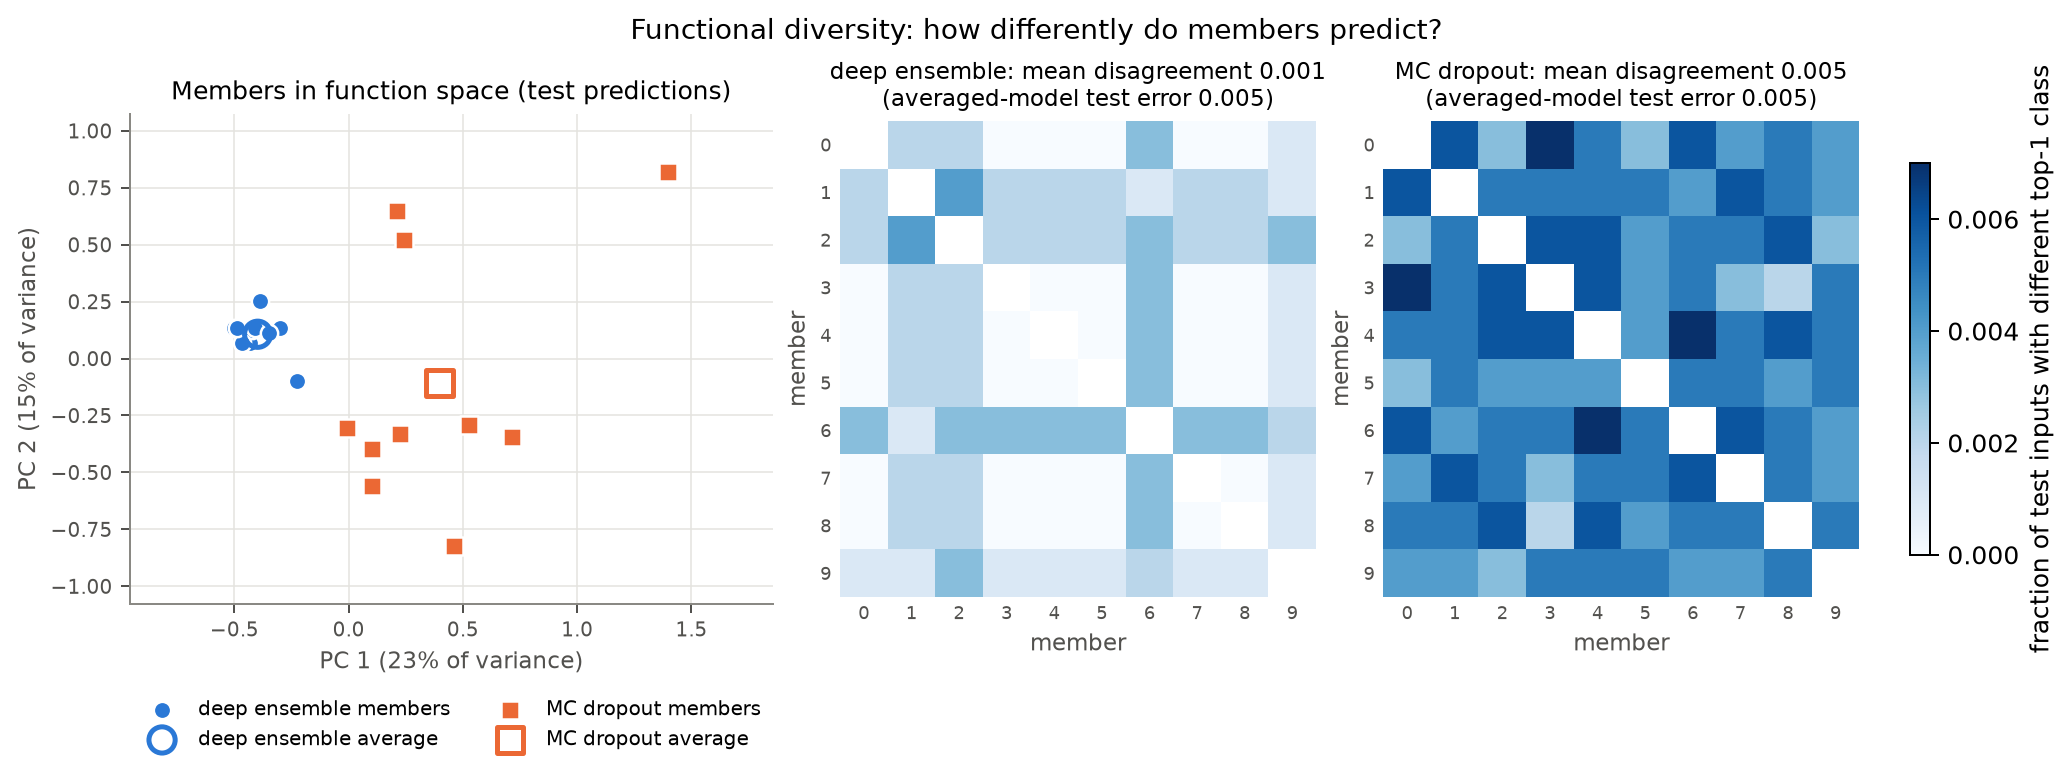
\includegraphics[width=\linewidth]{two_moons/figures/function_space.png}
  \caption{Two moons function space: members of both methods in one PCA of their test predictions (left) and pairwise top-1 disagreement (right).}
  \label{fig:tm-function}
\end{figure}

\FloatBarrier
\subsection{Fashion-MNIST}

\subsubsection{Training curves}

Both methods, DE and MC Dropout, were trained on Fashion-MNIST for 20 epochs, their training and test curves are shown in Figure~\ref{fig:fmnist-training}.
Both methods are trained to a near plateau by the end of training suggesting the models could have been trained longer, but the models did learn and we see no evidence of overfitting.
Unlike two moons, there is a clear gap between train and test performance (91.5\% vs.\ 88.7\% accuracy for the DE and 91.0\% vs.\ 88.4\% for MC Dropout).
Both methods reach similar final test performance with the DE slightly outperforming the MC Dropout in test accuracy (88.7\% vs. 88.4\%) and test NLL (0.318 vs.\ 0.332).

In contrast to two moons (Figure~\ref{fig:tm-training}), in which the ensemble and member-mean curves were nearly identical after the first few epochs, here the ensembles consistently outperform their average member.
Ensembling improves test accuracy by 1.22\% for the DE and 1.04\% for MC Dropout, and reduces NLL by 0.036 and 0.028 for DE and MC dropout respectively.
DE also shows a wider spread amongst its members, the standard deviation of member test accuracy is 0.33 percentage points, compared to 0.15 percentage points across MC dropout passes.
This wider gap between members reflect the epistemic uncertainty amongst members, suggesting Fashion-MNIST is serving as a more difficult evaluation benchmark when compared to two moons.

\begin{figure}[htbp]
  \centering
  \methodpair{fashion_mnist}{training_curves.png}
  \caption{Fashion-MNIST training curves: member mean $\pm1$ sd and the averaged prediction, on train and test.}
  \label{fig:fmnist-training}
\end{figure}

\subsubsection{Ensemble size}\label{sec:fmnist-size}

Figure~\ref{fig:fmnist-size} shows how each metric changes with respect to the number of members in the ensemble.
Unlike two moons, where the metrics largely remained flat, suggesting a single member had already sufficiently solved the task, both methods appear to now benefit from ensembling.
Test error decreases from 12.5\% to 11.3\% and 12.6\% to 11.6\% for DE and MC dropout respectively.
Similarly, DE and MC dropout have a respective decrease in test NLL of 0.354 to 0.318 and from 0.361 to 0.332.
For both methods we do see most of the improvement is gained by $k=5$ with a minimal improvement at  $k=10$.
Overall the DE continues to slightly outperform MC Dropout at every ensemble size.

Both predictive entropy and mutual information increase with $K$, which is expected as we anticipate more member disagreement leading to a less confident prediction.
At $k=10$, MI reached 0.031 for the DE and 0.029 for MC dropout, far exceeding the MI observed in two moons of 0.0003 and 0.0046 for DE and MC dropout respectively.
For both methods MI is about 8–10\% of predictive entropy suggesting most uncertainty of this task is aleatoric which is consistent with the complexity in the increase in classes and difficulty in distinguishing them.

Calibration is the exception to the observed steady improvement in other metrics.
Test ECE decreases from 0.019 (DE) and 0.012 (MC Dropout) for $k=1$ to 0.008 for both methods at $k=5$ and then slightly increases at $k=10$.
We observe that $k=1$ members are overconfident on the test set (the mean confidence exceeds accuracy by ~1.7 and 1.0 percentage points for DE and MC dropout), whereas by $k=5$ both methods are slightly underconfident (-0.4 and -0.6) and then grow to -0.8 points for both.
Test ECE is therefore the lowest at the point where we move from being overconfidant to underconfidant somewhere between $K=2$ and $k=5$.
We examine calibration in more detail with the reliability diagrams in Section~\ref{sec:fmnist-reliability}.

\begin{figure}[htbp]
  \centering
  \methodpair{fashion_mnist}{size_sweep.png}
  \caption{Fashion-MNIST metrics vs.\ number of members; error bars are $\pm1$ sd over $k$-member subsets.}
  \label{fig:fmnist-size}
\end{figure}

\subsubsection{Reliability}\label{sec:fmnist-reliability}
Figure~\ref{fig:fmnist-reliability} shows the reliability of each method on the test set comparing a single member to the the full $k=10$ ensemble.
This plot uses the same 15 confidence bins used for ECE and plots each bin's accuracy against its mean confidence.
For both methods, the majority of test input, roughly 60\%, fall into the highest confidence bin.
This diagram shows the same shift from over- to underconfidence observed in Section~\ref{sec:fmnist-size}.
Both single members list mostly below the diagonal for confidences between 0.6 and 0.95, thus they are overconfident.
After averaging, both method $k=10$ ensembles shift slightly above the diagonal in this range.
Ensembling therefore corrects the overconfidence of single members but slightly overshoots into underconfidence for both methods.


\begin{figure}[htbp]
  \centering
  \methodpair{fashion_mnist}{reliability.png}
  \caption{Fashion-MNIST test reliability: single member vs.\ full ensemble. Points below the diagonal are overconfident; the histogram shows each bin's share of inputs.}
  \label{fig:fmnist-reliability}
\end{figure}

\subsubsection{Function space}
Figure~\ref{fig:fmnist-function} shows the same function space view as for two moons.
The first principal component separates the two methods which is expected as the networks were trained independently.
As opposed to two moons, the DE members have a larger spread than MC dropout.
We believe this is primarily a reflection of the 2-D projection itself rather than a lack of diversity amongst MC dropout members.
The two components explain 33\% of the total variance, mostly the separation between the methods and the spread of the DE members.
About 27\% of DE member spread is captured but only 0.1\% of the MC dropout spread.

The disagreement matrices show a projection-free view of the diversity.
Unlike two moons, the DE now disagrees more than MC dropout with a mean pairwise disagreement of 7.5\% vs. 6.3\%, consistent with its slightly higher MI in Section~\ref{sec:fmnist-size}.
Both are far above the 0.5\% and 0.1\% observed with two moons.
We also see a large difference in member disagreement range, DE pairs range from 5.6\% to 9.8\% disagreement, whereas MC Dropout pairs are nearly uniform with a range of 5.9\% to 6.7\%.
This intuitively makes sense as DE members are trained independently and whereas MC dropout shares the same weights with smaller variations in activations.

\begin{figure}[htbp]
  \centering
  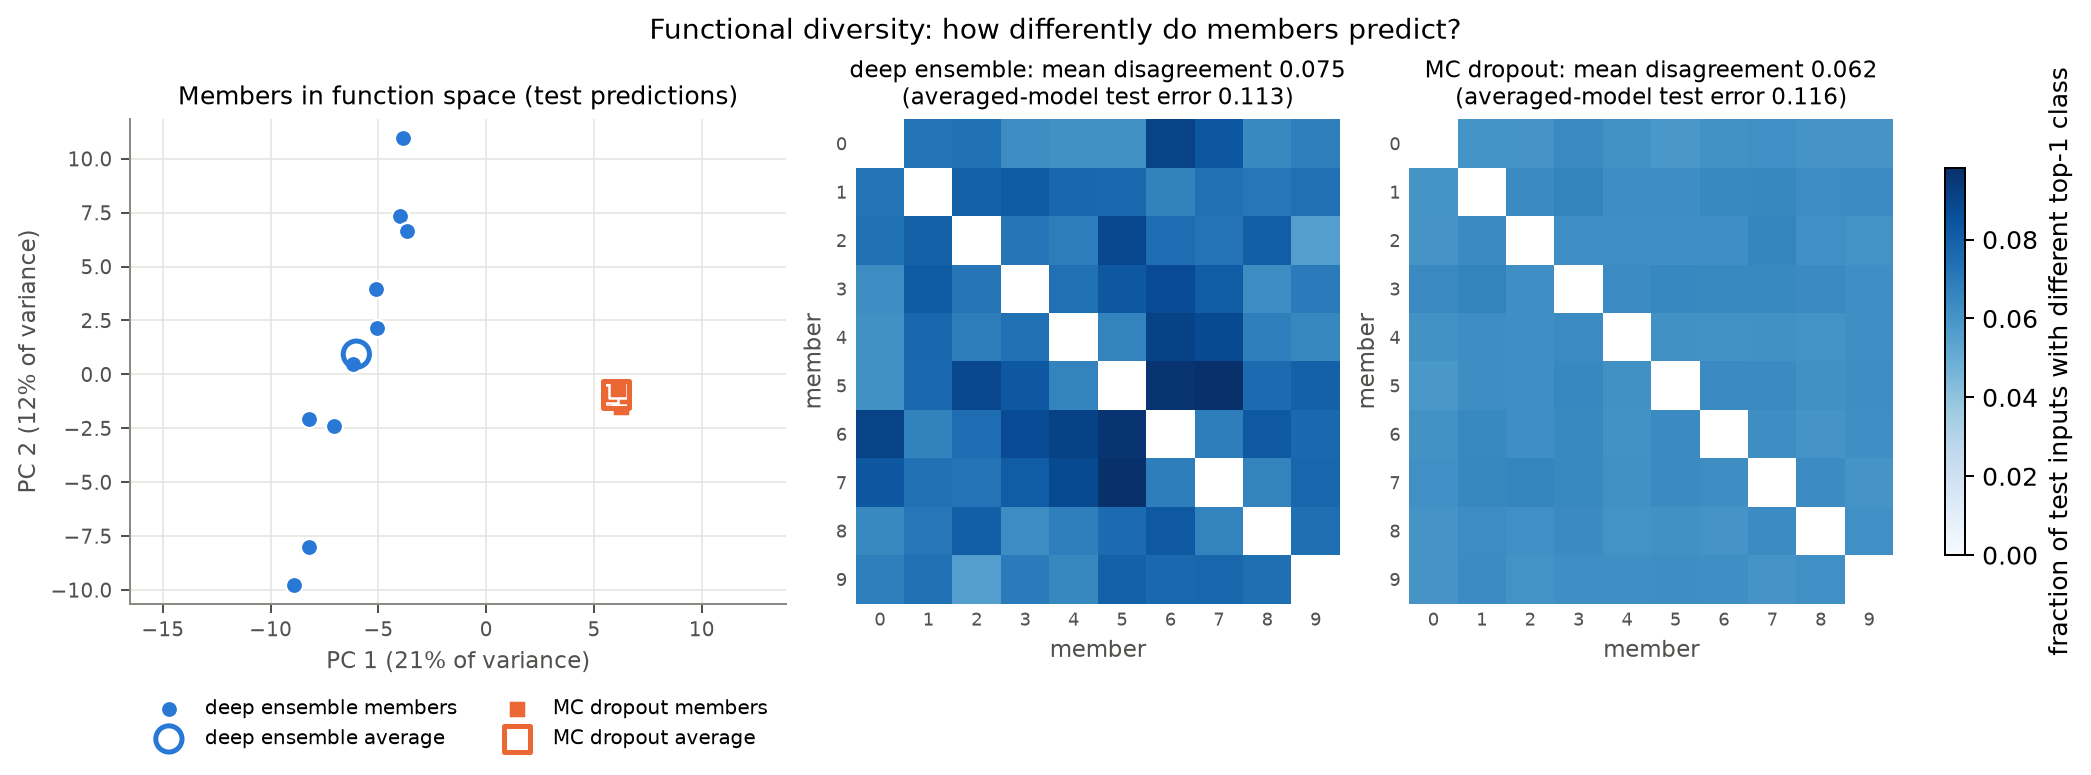
\includegraphics[width=\linewidth]{fashion_mnist/figures/function_space.png}
  \caption{Fashion-MNIST function space: members of both methods in one PCA of their test predictions (left) and pairwise top-1 disagreement (right).}
  \label{fig:fmnist-function}
\end{figure}

\section{Discussion and Conclusion}
  Across both datasets, single members of the two methods perform very similarly and the full ensembles are close.
  Neither method is consistently more diverse.
  On two moons, MC Dropout passes disagree more than DE members (0.5\% vs. 0.1\%), whereas on Fashion-MNIST the order reverses (6.3\% vs. 7.5\%).
  Which method produces more diverse members therefore depends on the task and likely the dropout rate and MLP architecture rather than the method alone.

  A further line of investigation would be to see how adjusting the dropout rate for MC dropout affects these observations or if we can find consistency across tasks.
  We observed that ensembling only helps when the task is sufficiently complex enough such that the members can disagree.
  Two moons is easy enough that a single member already solves it, so adding members did not see any benefit.
  Whereas on Fashion-MNIST, both methods improve with $K$.

  Ensembles allow us to separate uncertainty each member has from the uncertainty caused by their disagreement.
  On two moons MI is low on the trained data but rises as we move away from the data, as expected for epistemic uncertainty.
  For Fashion-MNIST, MI is only about 8--10\% of the predictive entropy for both methods, so most of the uncertainty is aleatoric.
  On Fashion-MNIST, averaging also corrects the overconfidence of single members, but beyond $k=5$ both methods become slightly underconfident.

\end{document}
